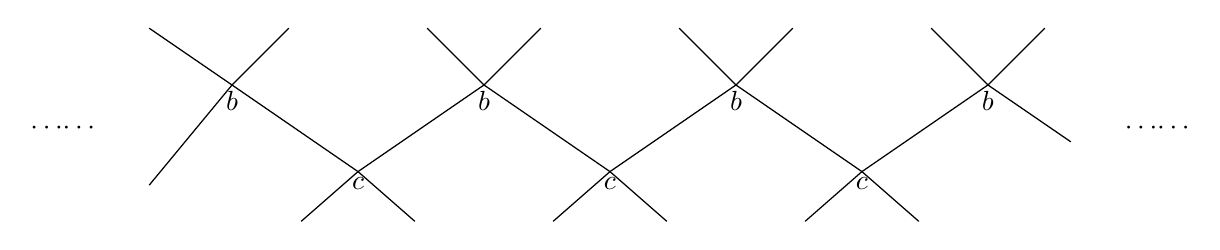
\begin{tikzpicture}[
  x=1cm,
  y=1cm,
  line cap=round,
  line join=round,
  every node/.style={inner sep=1pt}
]
  \coordinate (b1) at (2.8,0.55);
  \coordinate (c1) at (4.4,-0.55);
  \coordinate (b2) at (6.0,0.55);
  \coordinate (c2) at (7.6,-0.55);
  \coordinate (b3) at (9.2,0.55);
  \coordinate (c3) at (10.8,-0.55);
  \coordinate (b4) at (12.4,0.55);

  \draw[line width=.45pt]
    (1.75,1.27) -- (b1) -- (c1) -- (b2) -- (c2) --
    (b3) -- (c3) -- (b4) -- (13.45,-0.17);
  \draw[line width=.45pt] (1.75,-0.72) -- (b1) -- (3.52,1.27);
  \draw[line width=.45pt] (3.68,-1.18) -- (c1) -- (5.12,-1.18);
  \draw[line width=.45pt] (5.28,1.27) -- (b2) -- (6.72,1.27);
  \draw[line width=.45pt] (6.88,-1.18) -- (c2) -- (8.32,-1.18);
  \draw[line width=.45pt] (8.48,1.27) -- (b3) -- (9.92,1.27);
  \draw[line width=.45pt] (10.08,-1.18) -- (c3) -- (11.52,-1.18);
  \draw[line width=.45pt] (11.68,1.27) -- (b4) -- (13.12,1.27);

  \node[below=1pt] at (b1) {$b$};
  \node[below=1pt] at (b2) {$b$};
  \node[below=1pt] at (b3) {$b$};
  \node[below=1pt] at (b4) {$b$};
  \node[below=1pt] at (c1) {$c$};
  \node[below=1pt] at (c2) {$c$};
  \node[below=1pt] at (c3) {$c$};

  \node at (0.65,0) {$\cdots\!\cdots$};
  \node at (14.55,0) {$\cdots\!\cdots$};
\end{tikzpicture}
